% ============================================
% 软件工程大作业：基于 MVC 架构的命令行井字棋游戏
% 水电2401班 - 苏怡萌 - U202411889
% ============================================
\documentclass[12pt,a4paper]{ctexart}

% ---------- 页面设置 ----------
\usepackage[top=2.5cm, bottom=2.5cm, left=2.8cm, right=2.8cm]{geometry}
\usepackage{graphicx}
\usepackage{hyperref}
\usepackage{enumitem}
\usepackage{caption}
\usepackage{float}
\usepackage{fancyhdr}
\usepackage{titlesec}
\usepackage{xcolor}

% ---------- 超链接设置 ----------
\hypersetup{
    colorlinks=true,
    linkcolor=blue,
    urlcolor=blue,
    citecolor=blue
}

% ---------- 页眉页脚 ----------
\pagestyle{fancy}
\fancyhf{}
\fancyhead[L]{\small 软件工程大作业}
\fancyhead[R]{\small 水电2401班 苏怡萌}
\fancyfoot[C]{\thepage}
\renewcommand{\headrulewidth}{0.5pt}

% ---------- 标题格式 ----------
\titleformat{\section}{\Large\bfseries}{\thesection}{1em}{}
\titleformat{\subsection}{\large\bfseries}{\thesubsection}{1em}{}

\begin{document}

% ==================== 封面 ====================
\begin{titlepage}
    \centering
    \vspace*{3cm}
    
    {\Huge\bfseries 软件工程大作业\par}
    \vspace{1cm}
    {\LARGE 基于 MVC 架构的命令行井字棋游戏\par}
    
    \vspace{3cm}
    
    {\large
    \begin{tabular}{rl}
        \textbf{姓名：} & 苏怡萌 \\
        \textbf{学号：} & U202411889 \\
        \textbf{班级：} & 水电2401班 \\
        \textbf{日期：} & 2026年7月 \\
    \end{tabular}
    \par}
    
    \vspace{2cm}
    
    {\normalsize
    代码仓库：\url{https://github.com/Tim-dog/Software-Engineering-Major-Assignment}
    \par}
    
    \vfill
\end{titlepage}

% ==================== 目录 ====================
\tableofcontents
\newpage

% ==================== 1. 需求描述 ====================
\section{需求描述}

本项目要求使用 C++ 语言设计并实现一个\textbf{命令行版井字棋游戏}，采用经典的 $3\times 3$ 棋盘：
\begin{itemize}[itemsep=3pt]
    \item 两名玩家轮流在棋盘上落子
    \item 任意一方率先在横向、纵向或对角线上形成连续三个相同棋子即获胜
    \item 如果棋盘被填满且无人获胜，则游戏判定为平局
\end{itemize}

\textbf{架构要求}：采用 \textbf{MVC（Model-View-Controller）} 架构进行设计与实现。

\textbf{功能要求}：
\begin{itemize}[itemsep=3pt]
    \item 支持\textbf{双人对战}模式
    \item 支持\textbf{人机对战}模式（AI 自动选择第一个可落子的空格）
    \item 玩家通过命令行输入棋盘的行号和列号完成落子
\end{itemize}

\textbf{运行环境}：Windows + Visual Studio / VSCode，C++20 标准。

% ==================== 2. 系统设计 ====================
\section{系统设计}

\subsection{MVC 架构划分}

本项目严格遵循 MVC 三层架构：

\begin{table}[H]
\centering
\caption{MVC 架构层次与职责}
\begin{tabular}{|c|c|p{8cm}|}
\hline
\textbf{层次} & \textbf{类} & \textbf{职责} \\
\hline
\multirow{3}{*}{Model} & \texttt{Board} & 棋盘状态管理：落子、判满、查询 \\
\cline{2-3}
                       & \texttt{Player / HumanPlayer / AIPlayer} & 玩家抽象：人类输入、AI 决策（策略模式） \\
\cline{2-3}
                       & \texttt{Game} & 游戏核心逻辑：胜负判断、回合切换、状态机 \\
\hline
View & \texttt{BoardView} & 命令行界面渲染：棋盘绘制、状态显示 \\
\hline
Controller & \texttt{GameController} & 游戏主循环、协调 View 与 Model 的交互 \\
\hline
\end{tabular}
\end{table}

\subsection{关键设计决策}

\begin{enumerate}[itemsep=3pt]
    \item \textbf{玩家 X 始终由人类控制}：在人机模式下，AI 固定为玩家 O，简化设计
    \item \textbf{简单 AI 策略}：从左到右、从上到下扫描第一个空格子
    \item \textbf{输入校验}：\texttt{HumanPlayer::play()} 循环等待合法输入，支持格式错误、越界、占位三种异常处理
    \item \textbf{游戏结束状态}：\texttt{gameOver\_ + draw\_ + winner\_} 三个标志完整覆盖胜负/平局/进行中三种状态
\end{enumerate}

% ==================== 3. UML 建模 ====================
\section{UML 建模}

\subsection{用例图}

用例图如图~\ref{fig:usecase} 所示。玩家 1 负责开始游戏、选择模式和落子；玩家 2 或 AI 负责落子。落子操作包含胜负判断和回合切换。

\begin{figure}[H]
    \centering
    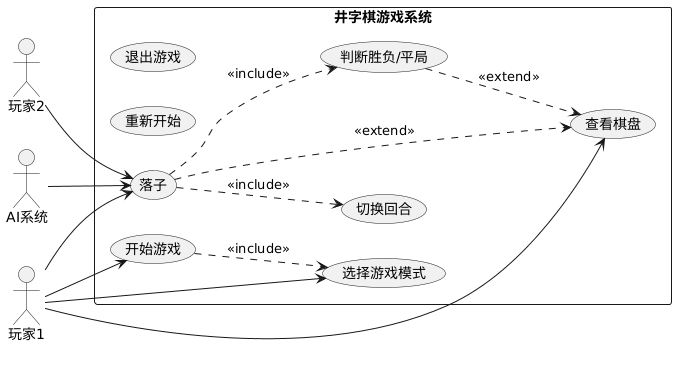
\includegraphics[width=0.85\textwidth]{figures/use_case.png}
    \caption{用例图}
    \label{fig:usecase}
\end{figure}

\subsection{类图}

类图如图~\ref{fig:class} 所示。Model 层包含 \texttt{Board}、\texttt{Player}（及其子类 \texttt{HumanPlayer}、\texttt{AIPlayer}）和 \texttt{Game}；View 层为 \texttt{BoardView}；Controller 层为 \texttt{GameController}。\texttt{Player} 为抽象类，使用多态实现人类与 AI 的差异化落子。

\begin{figure}[H]
    \centering
    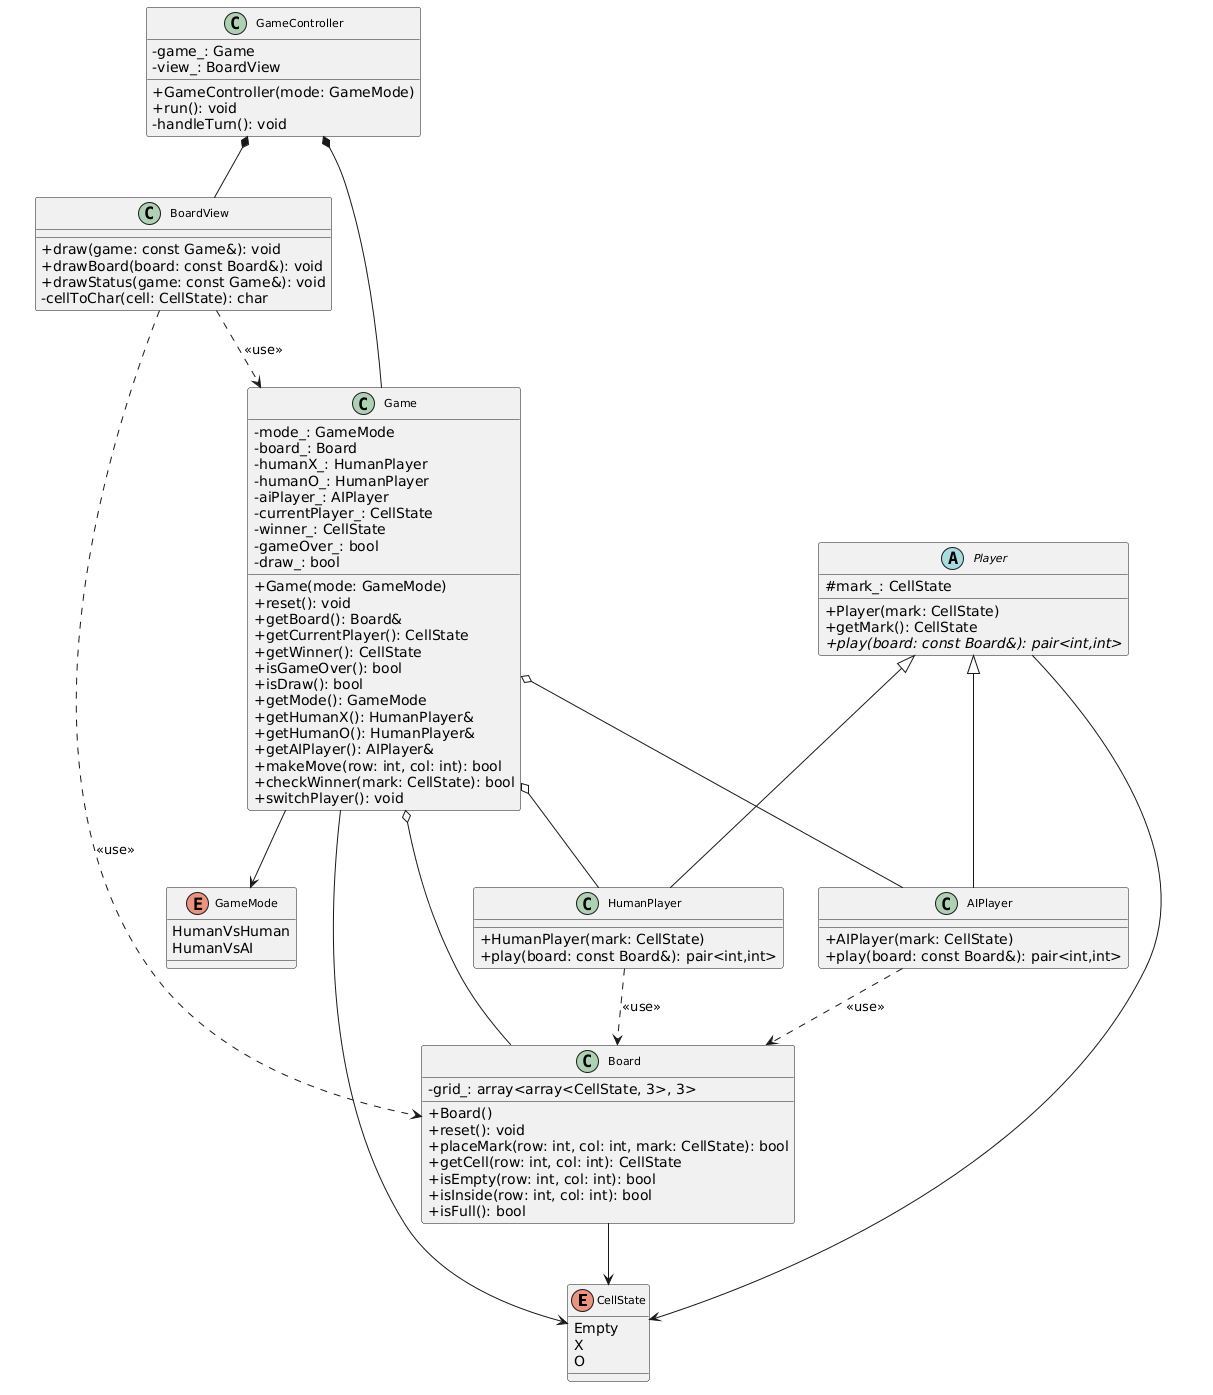
\includegraphics[width=1.0\textwidth]{figures/class_diagram.png}
    \caption{类图（MVC 架构）}
    \label{fig:class}
\end{figure}

\subsection{序列图}

序列图如图~\ref{fig:sequence} 所示。展示了双人对战模式下从游戏初始化到结束的完整消息序列，包含玩家 X、玩家 O、GameController、BoardView、Game、Board 六个参与者的交互。

\begin{figure}[H]
    \centering
    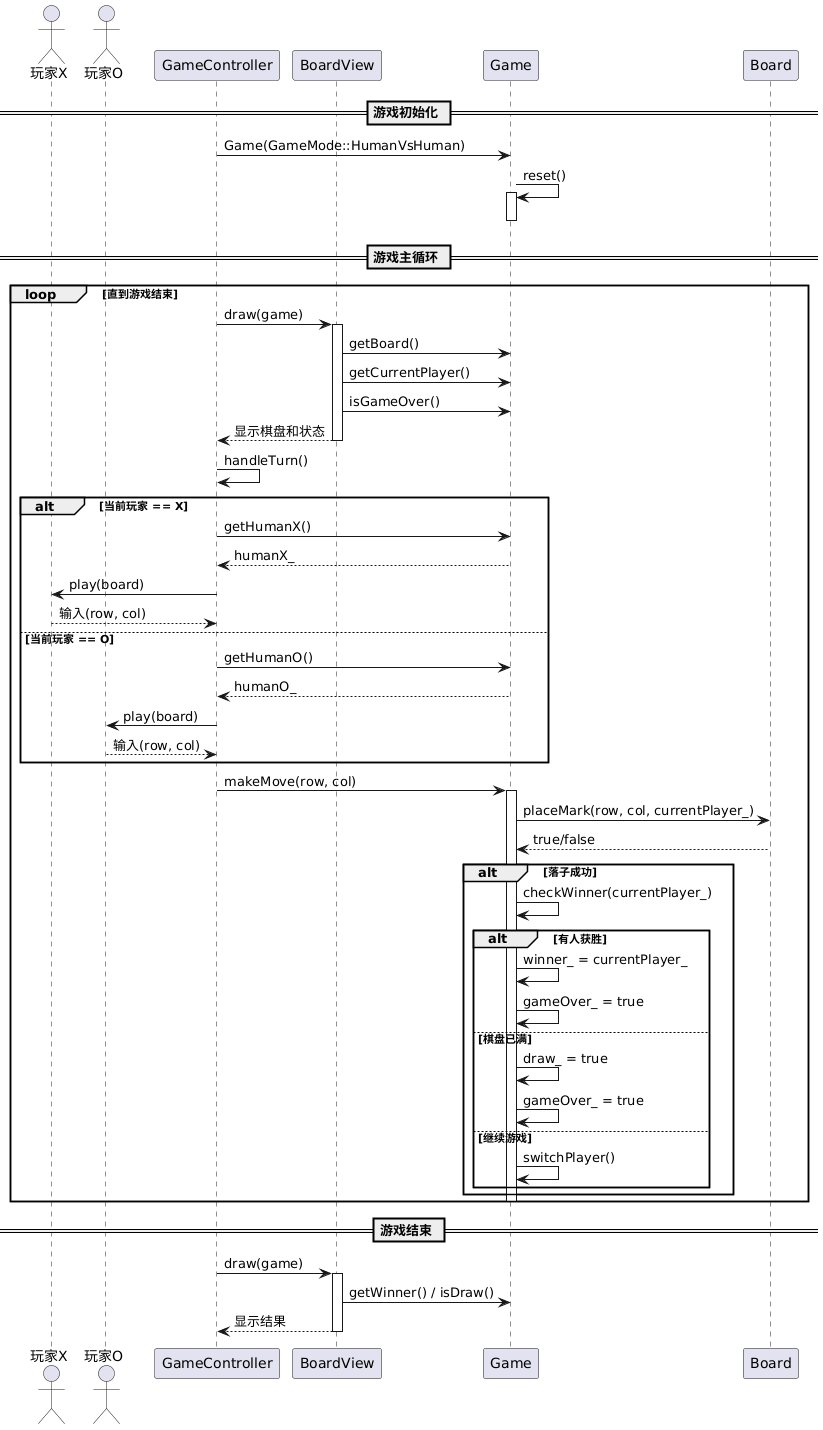
\includegraphics[width=0.95\textwidth]{figures/sequence_diagram.png}
    \caption{序列图（双人对战流程）}
    \label{fig:sequence}
\end{figure}

% ==================== 4. 模块划分与类职责 ====================
\section{模块划分与类职责}

\subsection{Model 层}

\subsubsection{Board（棋盘类）}
\textbf{职责}：维护 $3\times 3$ 棋盘状态，提供落子、查询、判满等原子操作。\\
\textbf{关键方法}：
\begin{itemize}[itemsep=2pt]
    \item \texttt{placeMark(row, col, mark)} — 在指定位置落子，返回是否成功
    \item \texttt{getCell(row, col)} — 获取指定格子的棋子状态
    \item \texttt{isEmpty(row, col) / isInside(row, col)} — 边界和空位检查
    \item \texttt{isFull()} — 判断棋盘是否已满（用于平局判断）
\end{itemize}

\subsubsection{Player / HumanPlayer / AIPlayer（玩家类族）}
\textbf{职责}：抽象玩家行为，通过多态支持人类输入和 AI 决策。\\
\textbf{设计模式}：策略模式 — \texttt{Player} 为抽象基类，\texttt{play()} 为纯虚函数。
\begin{itemize}[itemsep=2pt]
    \item \texttt{HumanPlayer::play()} — 循环读取命令行输入，校验格式/范围/占用后返回坐标
    \item \texttt{AIPlayer::play()} — 从左到右、从上到下扫描首个空格子
\end{itemize}

\subsubsection{Game（游戏核心类）}
\textbf{职责}：管理游戏状态机，协调 Board 和 Player，判断胜负和平局。\\
\textbf{关键方法}：
\begin{itemize}[itemsep=2pt]
    \item \texttt{makeMove(row, col)} — 执行一步落子的完整流程（落子→判胜→判平→切换回合）
    \item \texttt{checkWinner(mark)} — 检查 3 行、3 列、2 条对角线是否三连
    \item \texttt{switchPlayer()} — 在 X 和 O 之间切换当前玩家
\end{itemize}

\subsection{View 层}

\subsubsection{BoardView（视图类）}
\textbf{职责}：在命令行中渲染棋盘、当前玩家信息、游戏结果。\\
\textbf{关键方法}：
\begin{itemize}[itemsep=2pt]
    \item \texttt{draw(game)} — 绘制完整界面（棋盘 + 状态）
    \item \texttt{drawBoard(board)} — 绘制 $3\times 3$ 网格棋盘
    \item \texttt{drawStatus(game)} — 显示当前回合或游戏结果
    \item \texttt{cellToChar(cell)} — 将 \texttt{CellState} 枚举转换为显示字符
\end{itemize}

\subsection{Controller 层}

\subsubsection{GameController（控制器类）}
\textbf{职责}：驱动游戏主循环，协调 View 和 Model 的交互。\\
\textbf{关键方法}：
\begin{itemize}[itemsep=2pt]
    \item \texttt{run()} — 游戏主循环：画界面 → 处理回合 → 检查结束
    \item \texttt{handleTurn()} — 根据当前模式和玩家选择合适的 Player 对象，调用 \texttt{play()} 获取坐标，调用 \texttt{makeMove()} 执行落子
\end{itemize}

\subsection{配置}

\texttt{Config.h} 定义了全局配置：
\begin{itemize}[itemsep=2pt]
    \item \texttt{BOARD\_SIZE = 3} — 棋盘大小常量
    \item \texttt{CellState} 枚举 — \texttt{Empty}, \texttt{X}, \texttt{O}
    \item \texttt{GameMode} 枚举 — \texttt{HumanVsHuman}, \texttt{HumanVsAI}
\end{itemize}

\subsection{类之间的关系}

\begin{verbatim}
GameController ◆── Game           (组合：Controller 拥有 Game)
GameController ◆── BoardView      (组合：Controller 拥有 View)
Game ◆── Board                    (组合：Game 拥有 Board)
Game ◇── HumanPlayer              (聚合：Game 拥有 HumanPlayer 和 AIPlayer)
Player <|── HumanPlayer           (继承：HumanPlayer 是 Player 的子类)
Player <|── AIPlayer              (继承：AIPlayer 是 Player 的子类)
BoardView ..> Game                (依赖：View 读取 Game 状态)
BoardView ..> Board               (依赖：View 读取 Board 状态)
HumanPlayer ..> Board             (依赖：玩家读取 Board 选择落子位置)
AIPlayer ..> Board                (依赖：AI 读取 Board 选择落子位置)
\end{verbatim}

% ==================== 5. 游戏运行流程 ====================
\section{游戏运行流程}

游戏主流程如下：

\begin{enumerate}[itemsep=3pt]
    \item 程序启动，\texttt{main()} 设置 UTF-8 控制台编码，显示模式选择菜单
    \item 用户选择 1（双人对战）或 2（人机对战）
    \item \texttt{GameController} 初始化 \texttt{Game} 和 \texttt{BoardView} 对象
    \item 进入主循环 \texttt{while (!game\_.isGameOver())}：
    \begin{itemize}[itemsep=2pt]
        \item \texttt{BoardView::draw()} 绘制当前棋盘和状态
        \item \texttt{GameController::handleTurn()} 根据当前玩家和模式选择 \texttt{HumanPlayer} 或 \texttt{AIPlayer}，调用其 \texttt{play()} 获取落子坐标
        \item \texttt{Game::makeMove(row, col)} 执行落子、判断胜负、判断平局、切换回合
    \end{itemize}
    \item 游戏结束后显示最终结果（X 胜 / O 胜 / 平局）
    \item 按回车键退出程序
\end{enumerate}

% ==================== 6. 代码运行截图 ====================
\section{代码运行截图}

\subsection{程序启动界面（模式选择）}

\begin{figure}[H]
    \centering
    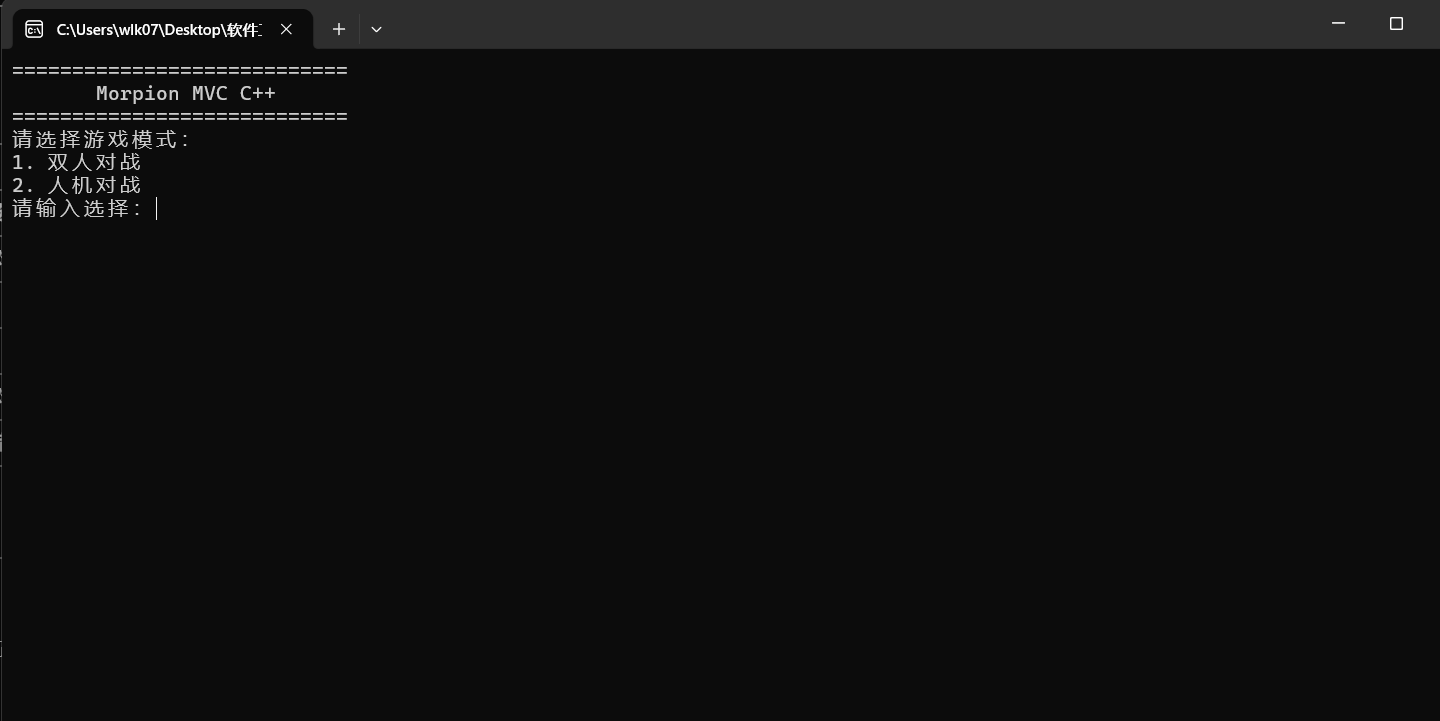
\includegraphics[width=0.80\textwidth]{软件运行情况截图/程序启动界面.png}
    \caption{程序启动界面 — 模式选择（1=双人对战，2=人机对战）}
    \label{fig:start}
\end{figure}

\subsection{双人对战进行中}

\begin{figure}[H]
    \centering
    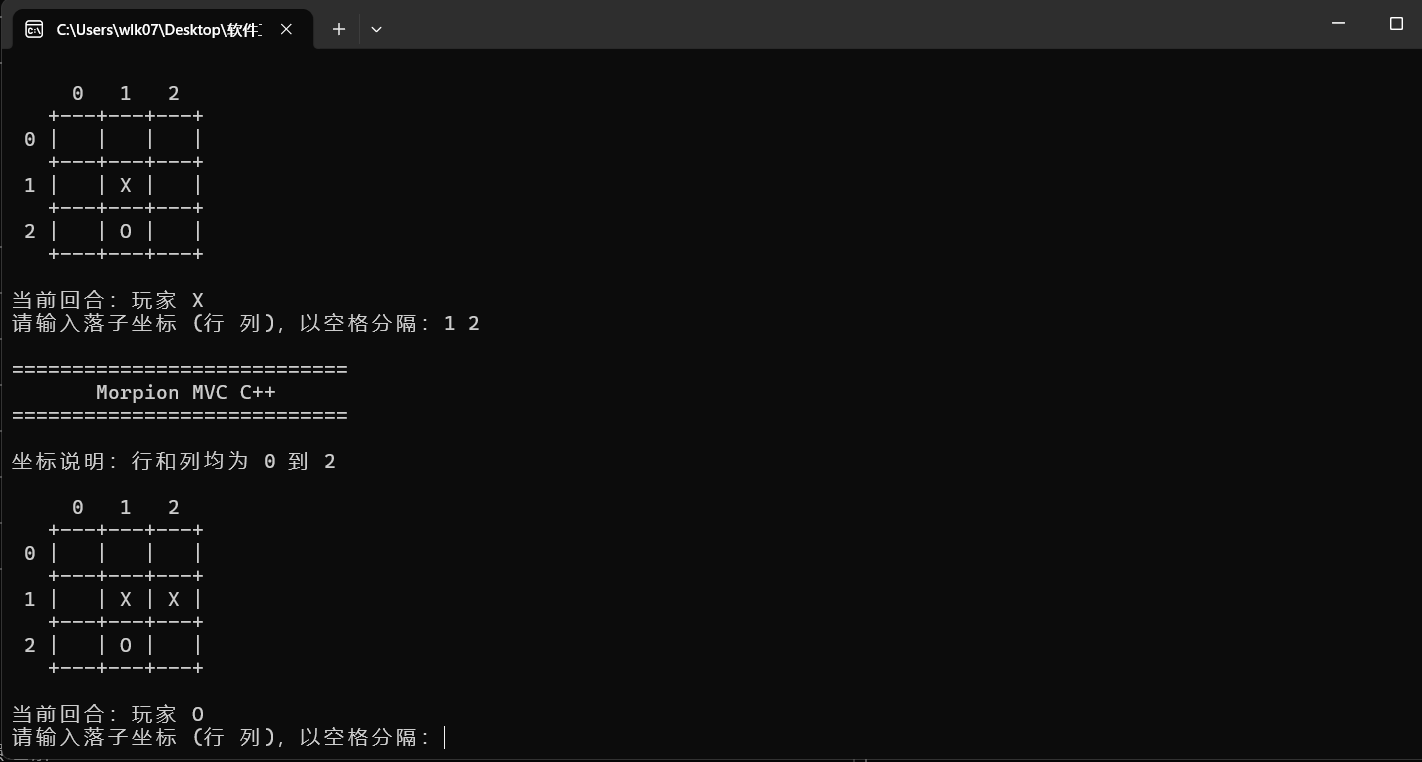
\includegraphics[width=0.80\textwidth]{软件运行情况截图/双人对战进行中.png}
    \caption{双人对战进行中 — X 与 O 交替落子}
    \label{fig:playing}
\end{figure}

\subsection{X 获胜}

\begin{figure}[H]
    \centering
    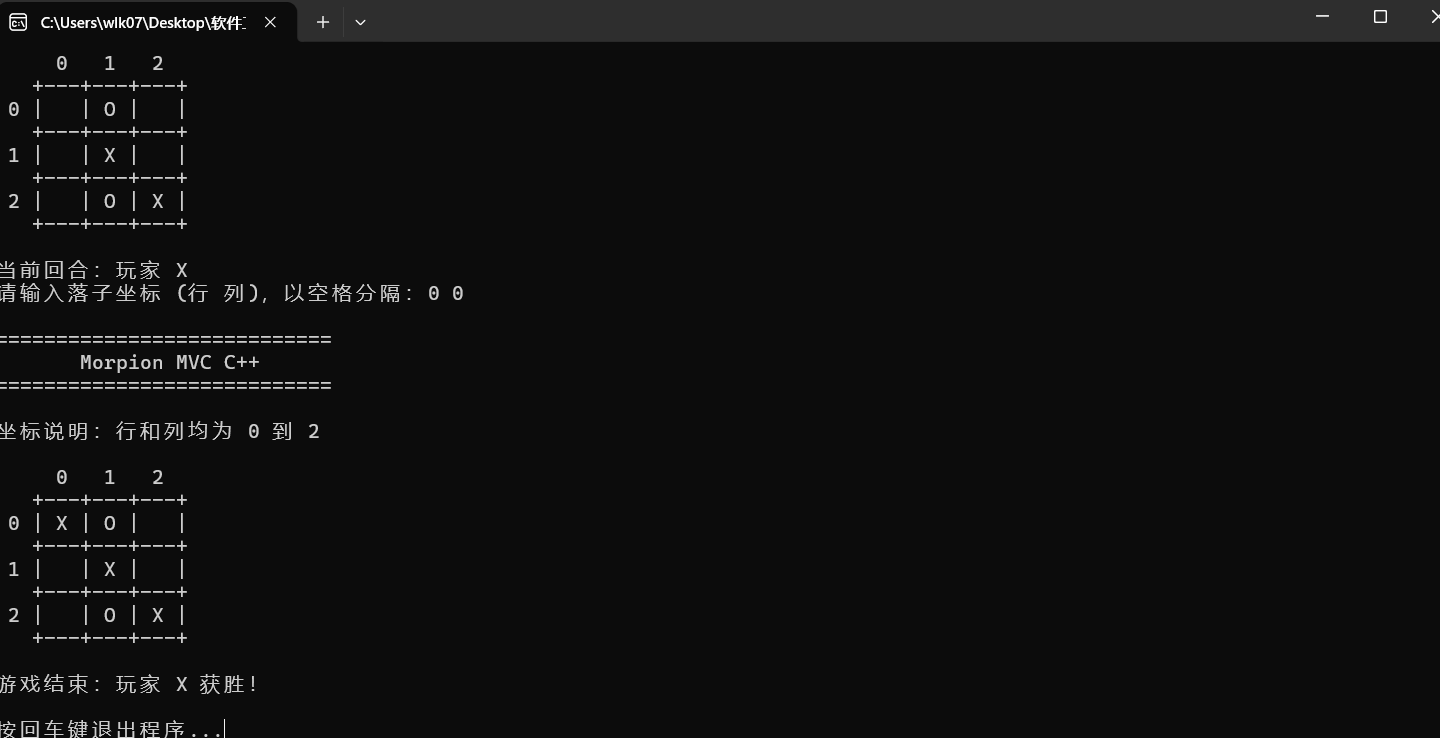
\includegraphics[width=0.80\textwidth]{软件运行情况截图/X获胜.png}
    \caption{X 获胜 — 横向三连}
    \label{fig:xwin}
\end{figure}

\subsection{平局}

\begin{figure}[H]
    \centering
    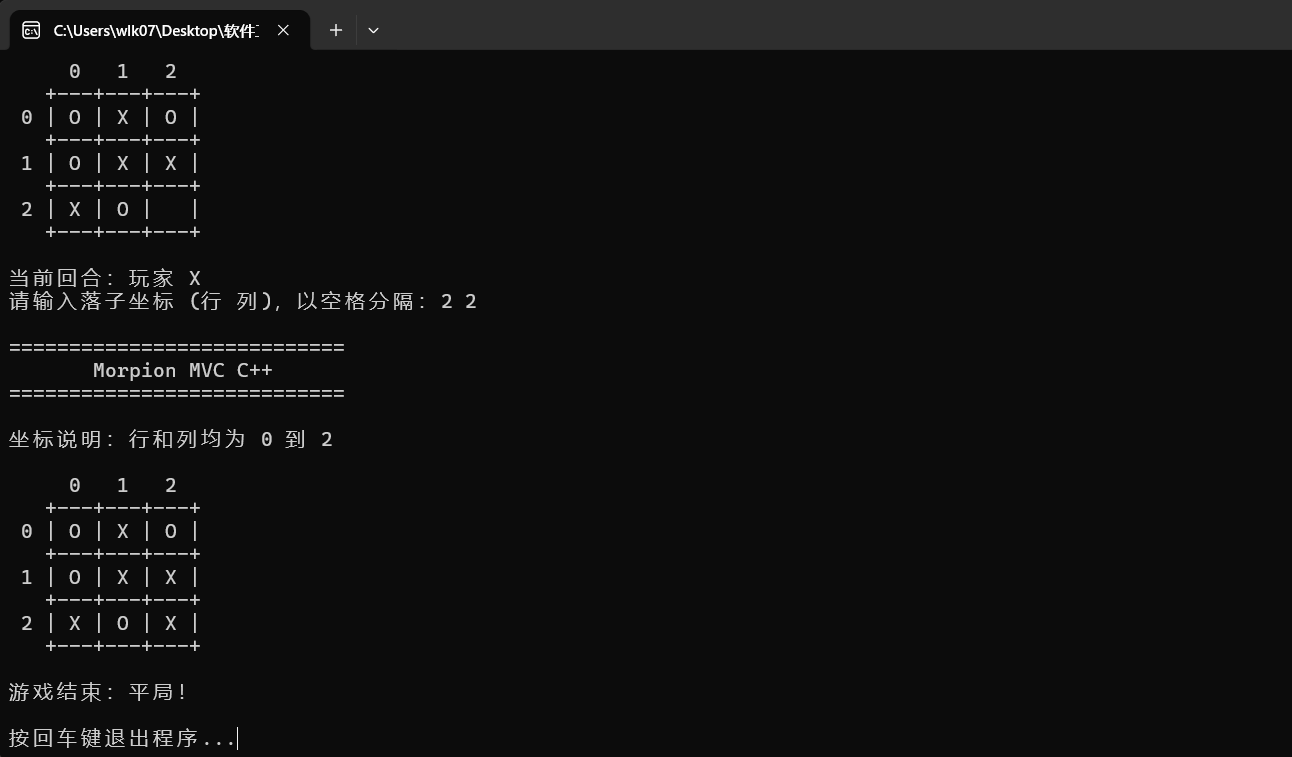
\includegraphics[width=0.80\textwidth]{软件运行情况截图/平局界面.png}
    \caption{平局 — 棋盘填满无人获胜}
    \label{fig:draw}
\end{figure}

\subsection{人机对战}

\begin{figure}[H]
    \centering
    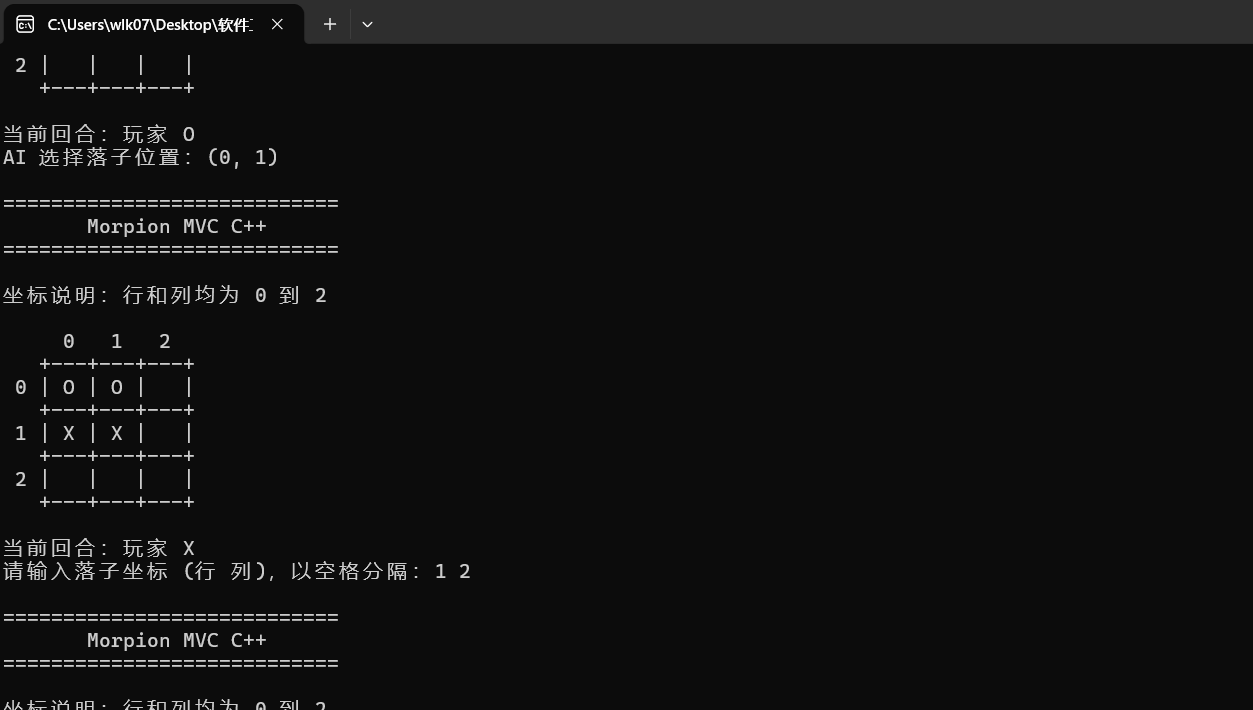
\includegraphics[width=0.80\textwidth]{软件运行情况截图/人机对战界面.png}
    \caption{人机对战 — AI 自动选择空格落子}
    \label{fig:ai}
\end{figure}

\subsection{不合法操作提示}

\begin{figure}[H]
    \centering
    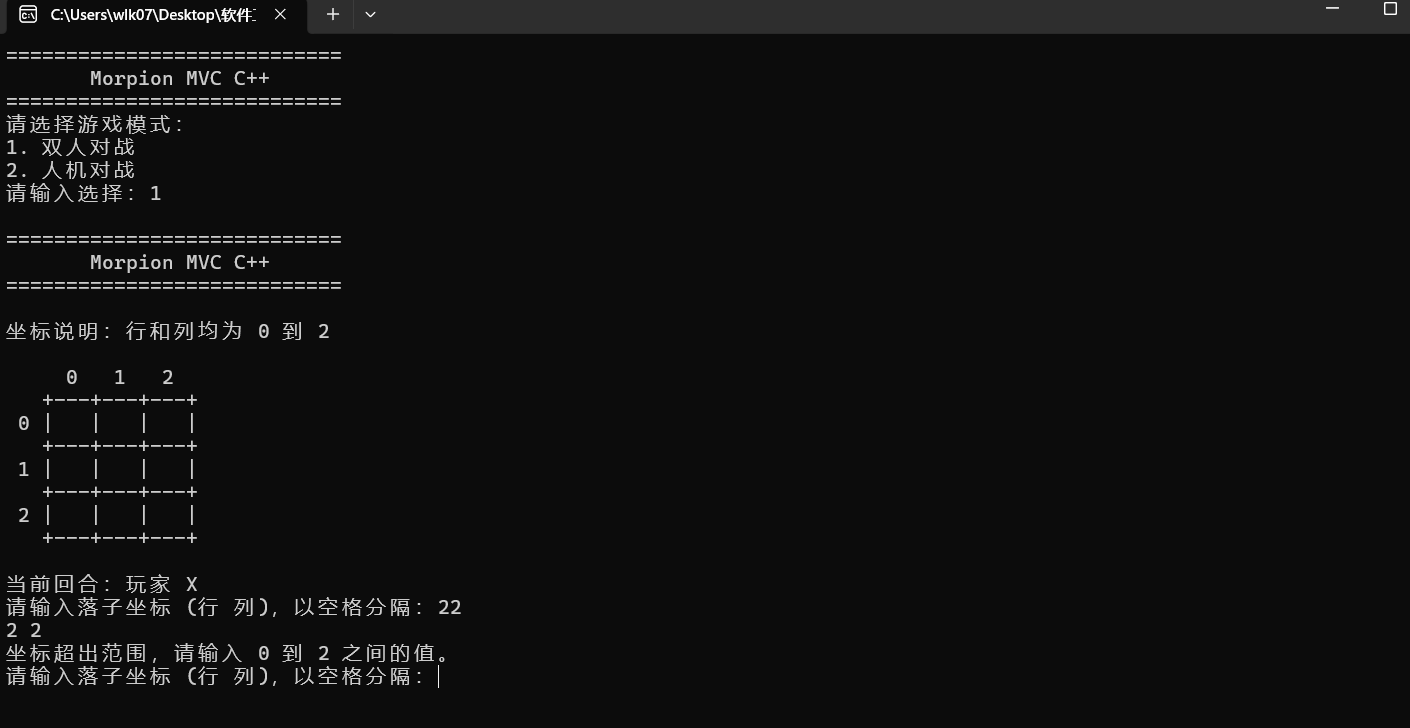
\includegraphics[width=0.80\textwidth]{软件运行情况截图/不合法操作.png}
    \caption{输入校验 — 坐标越界或格式错误的提示信息}
    \label{fig:invalid}
\end{figure}

% ==================== 7. 项目结构 ====================
\section{项目结构}

\begin{verbatim}
ProjectMorpion/
├── main.cpp                  # 程序入口，模式选择 + UTF-8 控制台设置
├── Config.h                  # 全局配置（BOARD_SIZE、CellState、GameMode 枚举）
├── Board.h / Board.cpp       # Model: 棋盘状态管理
├── Player.h / Player.cpp     # Model: 玩家抽象类 + HumanPlayer + AIPlayer
├── Game.h / Game.cpp         # Model: 游戏核心逻辑
├── BoardView.h / BoardView.cpp  # View: 命令行界面渲染
├── GameController.h / GameController.cpp  # Controller: 游戏主循环和回合控制
├── ProjectMorpion.slnx       # Visual Studio 解决方案文件
├── ProjectMorpion.vcxproj    # Visual Studio 项目文件
├── .vscode/tasks.json        # VSCode 编译任务配置（Ctrl+Shift+B）
├── .gitignore                # Git 忽略规则
├── README.md                 # 项目说明文档
├── report.md                 # Markdown 版报告
├── docs/                     # UML 设计文档（PlantUML 源码）
│   ├── use_case.puml
│   ├── class_diagram.puml
│   └── sequence_diagram.puml
├── figures/                  # UML 渲染图片
├── scripts/                  # 辅助脚本
└── 软件运行情况截图/           # 游戏运行截图（6 张）
\end{verbatim}

代码仓库：\url{https://github.com/Tim-dog/Software-Engineering-Major-Assignment}

\end{document}
